\documentclass{beamer}
\usepackage{listings}
\usepackage{mdframed}
\usepackage{tikz}
\usepackage{pdfpages}
\usepackage[francais]{babel}
\usepackage[utf8]{inputenc}
\usepackage{float}
\usepackage{graphicx}
\usepackage{wrapfig}
\usepackage{times}
\usepackage[T1]{fontenc}
\usepackage[overlay,absolute]{textpos}

\newcommand{\firstlogo}{images/conti.png}
\newcommand{\secondlogo}{ups.jpg}
\newcommand{\thirdlogo}{mdl.png}
\newcommand{\footsubject}{Développement d'un outil de tests automatisés pour un logiciel de contrôle moteur} 
\newcommand{\rgbcolortheme}{230,146,26}

\makeatletter
\hypersetup{pdfpagemode=FullScreen}

\mode<presentation> {
	\usepackage{../beamer-theme/beamerthemeUNLTheme}
}

\title[] % (facultatif, \`a utiliser uniquement si le titre de l'article est trop long)
{Développement d'un outil de tests automatisés pour un logiciel de contrôle moteur}
\subtitle {}

\newcommand{\authors}{%
	\large
Antoine de \bsc{Roquemaurel}\newline
\scriptsize {
Universit\'e Toulouse III -- Paul Sabatier \\
M2 Informatique -- Développement Logiciel 
}
}

\author[
Antoine de \bsc{Roquemaurel}
]{\authors}

\institute[] 
{
	Maître de stage: Alain \bsc{Fernandez}\newline
	Tuteur universitaire: Jean-Baptiste \bsc{Raclet}

	\hspace{-15px}
	\includegraphics[height=0.8cm]{ups.jpg}
	\hfill
	\hspace{15px}
	\includegraphics[height=0.7cm]{mdl.png}
	\hfill
	\hspace{15px}
	\includegraphics[height=0.8cm]{images/conti.png}
	\vspace{-10px}
}

\date[ ~ ~ ~ 14 / 01 / 2016] % (facultatif, peut être une abr\'eviation du nom de la conf\'erence)
{Jeudi 14 Janvier 2016}

\pgfdeclareimage[width=2.5cm]{le-logo}{images/conti.png}
\logo{\pgfuseimage{le-logo}}


\AtBeginSection[] {
\begin{frame}<beamer>{Plan}
	\tableofcontents[currentsection]
\end{frame}
}

\setbeamerfont*{section in sidebar}{size=\fontsize{8px}{2.3em}\selectfont }
\setbeamerfont*{subsection in sidebar}{size=\fontsize{5px}{1.5em}\selectfont }
\begin{document}
	\sidetoc{no}
	\begin{frame}
		\titlepage
	\end{frame}

	%\chapter*{Introduction}
	\addcontentsline{toc}{chapter}{Introduction} 


Dans le cadre de ma formation en première année de Master spécialité Développement Logiciel à l'université Toulouse III – Paul Sabatier, j'ai eu la possibilité d'effectuer un stage.


Attiré par le monde de l'entreprise et désireux de gagner en expérience, j'ai eu l'opportunité de continuer un projet commencé l'année précédente lors de mon stage de fin de Licence dans l'entreprise Continental Automotive : le développement d'une plateforme de tests de logiciels embarqués.

Ce projet a pour but d'aider une équipe de Continental, celle-ci est en charge de l'intégration d'un plugin, fourni sous forme binaire, que l'équipe doit intégrer dans le logiciel d'un calculateur de contrôle moteur. Pour cela, une plateforme permettant d'effectuer des tests automatisés est en développement.

Ayant connu les prémices de ce projet, et afin d'avoir un aperçu de celui-ci sur la longueur, allant de sa conception jusqu'à sa mise en production, le sujet du stage était particulièrement intéressant. En outre, celui-ci est en parfaite adéquation avec mon projet professionnel, et ma poursuite en M2 Développement Logiciel.

C'est au sein de l'équipe \textit{Test \& Automation Service} que j'ai effectué mon stage d'une durée de quatre mois, je vais ainsi vous présenter en quoi le développement de cet outil est nécessaire à l'équipe en charge des tests de ce plugin. Dans une première partie nous présenterons l'entreprise Continental et plus particulièrement l'équipe Tests \& Automation Service(chapitres \ref{chapConti} et \ref{chapOrganization}). Nous aborderons ensuite le problème que posent actuellement les tests de ce plugin(chapitre \ref{chapPb}), avant de présenter la solution qui est en cours de développement(chapitre \ref{chapGreent}) et comment j'ai contribué à ce projet(chapitre \ref{collab}). 


	\sidetoc{yes}
	\section{L'entreprise} 
	\subsection{Continental}
\begin{frame}{L'entreprise Continental}

	\begin{itemize}
		\item Entreprise allemande
			\begin{itemize}
				\item Créée en 1871
				\item Plus de $189\;000$ employés\newline
				$\rightarrow$ Dont $2\;000$ à Toulouse
				\item Dans 50 pays différents
			\end{itemize}

			\begin{figure}[H]
				\only<1>{
					\hspace{-30px}
					\includegraphics[width=9.5cm]{images/repartition_conti.png}
									\caption{Répartition de Continental dans le monde}
				}
				\only<2>{
					\vspace{-10px}
					\includegraphics[width=6.5cm]{images/repartition_conti.png}
					\vspace{-10px}
					\caption{\scriptsize Répartition de Continental dans le monde}
				}

			\end{figure}
			\vfill				
		\only<2>{
								\vspace{-10px}
		\item Equipementier Automobile
			\begin{itemize}
				\item Pneus
				\item Sécurité Automobile
				\item Injecteurs
				\item Contrôle moteur
				\item \ldots			
			\end{itemize}
		}
	\end{itemize}
\end{frame}
\subsection{Le groupe Tests Automation Service}
\begin{frame}{Le groupe Tests Automation Service}

	\begin{itemize}
		\item Appartient à la division << \textit{Powertrain} >>
			\begin{itemize}
				\item Calculateurs de contrôle moteur
				\item Mise au point des systèmes essence ou diesel
			\end{itemize}
	\end{itemize}
	
	\vfill
	\pause
	\begin{block}{Le besoin}
		\begin{itemize}
			\item Système à haut risque 
			\item Très complexe
			\begin{itemize}
				\item Des milliers de variables
				\item Des milliers de pages de spécifications
			\end{itemize}
			$\Rightarrow$ Automatisation des tests indispensable
		\end{itemize}
	\end{block}
	\pause
	\begin{itemize}
		\item Le groupe doit fournir des services de tests :
			\begin{itemize}
				\item Tests d'intégration
				\item Tests de non régression
			\end{itemize}
	\end{itemize}
\end{frame}

	\section{Le projet}
	\subsection{Le problème}
	\begin{frame}{Le problème des tests}
	\begin{wrapfigure}{r}{4cm}
		\vspace{-60px}
		\begin{figure}[H]
		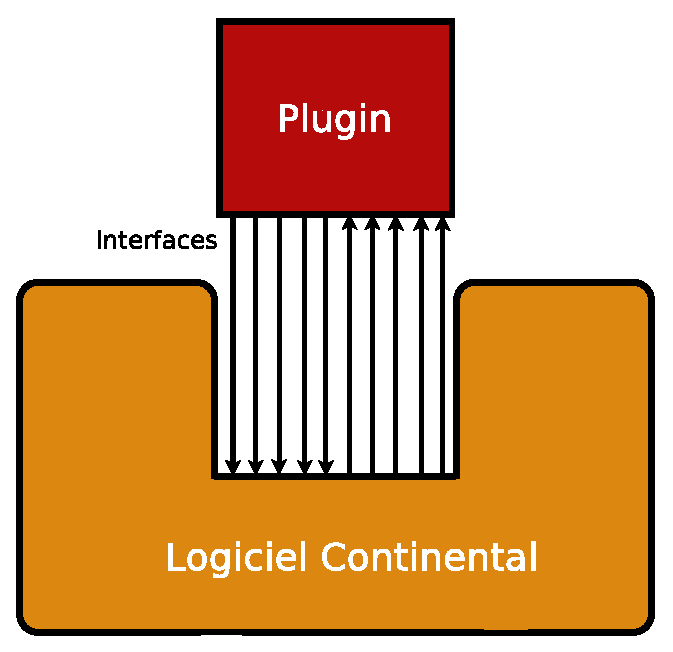
\includegraphics[width=3cm]{images/plugin.eps}
		\caption{\scriptsize Intégration du \textit{plugin}}
		\end{figure}		
	\end{wrapfigure}

	\vfill
	\vspace{-10px}
	\begin{minipage}{0.6\textwidth}
			Intégration du << plugin >>
			\begin{itemize}
				\item Fourni par le client
				\item Doit s'interfacer avec les logiciels Continental 
				\item Spécification des variables fournie au format Excel
			\end{itemize}
				\end{minipage}
			\pause
	\vfill	
	\vspace{20px}
	\begin{alertblock}{Difficile à tester}
		Tests manuels qui sont : 
		\begin{itemize}
			\item Non exhaustifs
			\item Longs à faire
			\item Répétitifs
		\end{itemize}
	\end{alertblock}
	\vfill
\end{frame}


	\subsection{La solution : GreenT} 
	\begin{frame}{Fonctionnalités de la solution : GreenT}
\vspace{-10px}
	\begin{itemize}
		\item Analyser le fichier de spécifications\newline
			\footnotesize
			$\rightarrow$ Fichier complété par un testeur au sein de Continental
			\normalsize

		\item Générer automatiquement des fichiers exécutables
		\item Rapports détaillés

	\end{itemize}
	\vfill
	\begin{figure}[H]
		\centering
		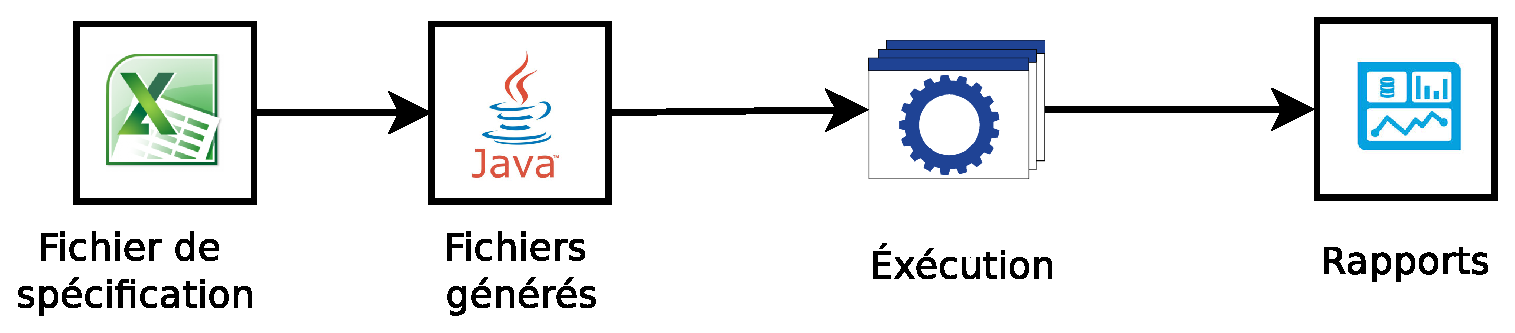
\includegraphics[width=8.5cm]{images/fct.eps}
		\caption{Fonctionnalités principales}
	\end{figure}
\end{frame}

\begin{frame}{Fonctionnement global de GreenT}
	\begin{figure}[H]
		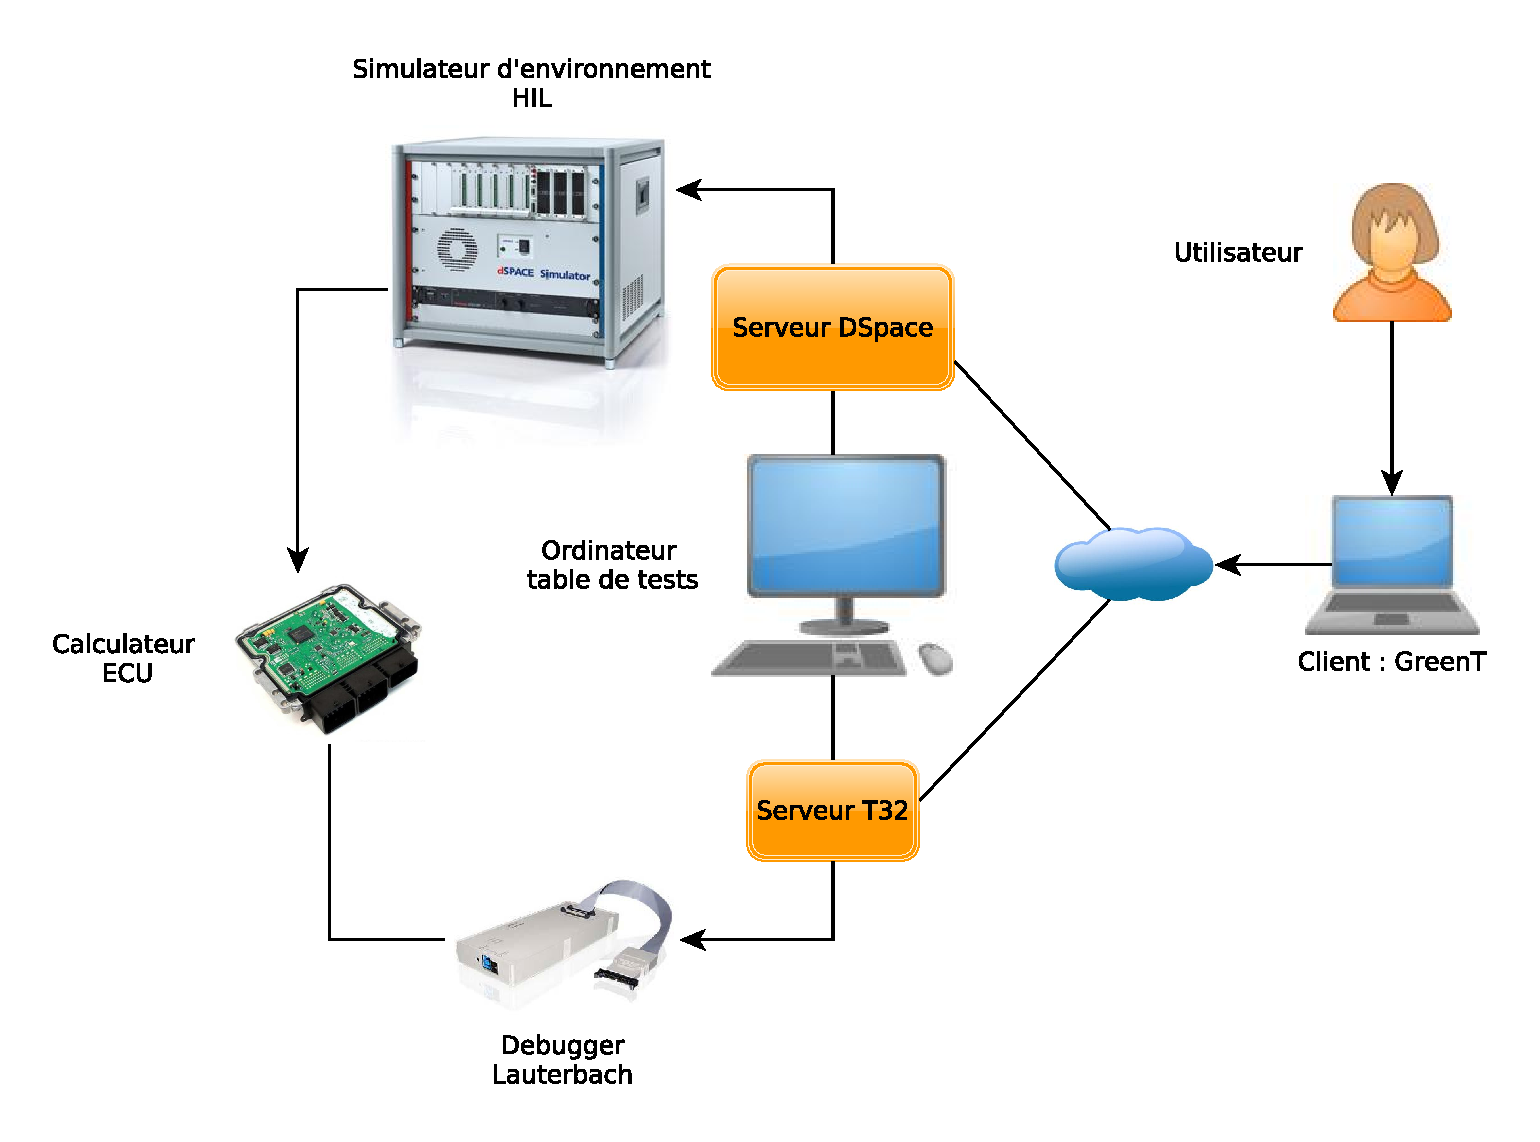
\includegraphics[width=9cm]{images/network.eps}
		\caption{Schéma de fonctionnement général}	
	\end{figure}
\end{frame}
\begin{frame}[plain]
	\begin{tikzpicture}[remember picture,overlay]
	\node[at=(current page.center)] {
		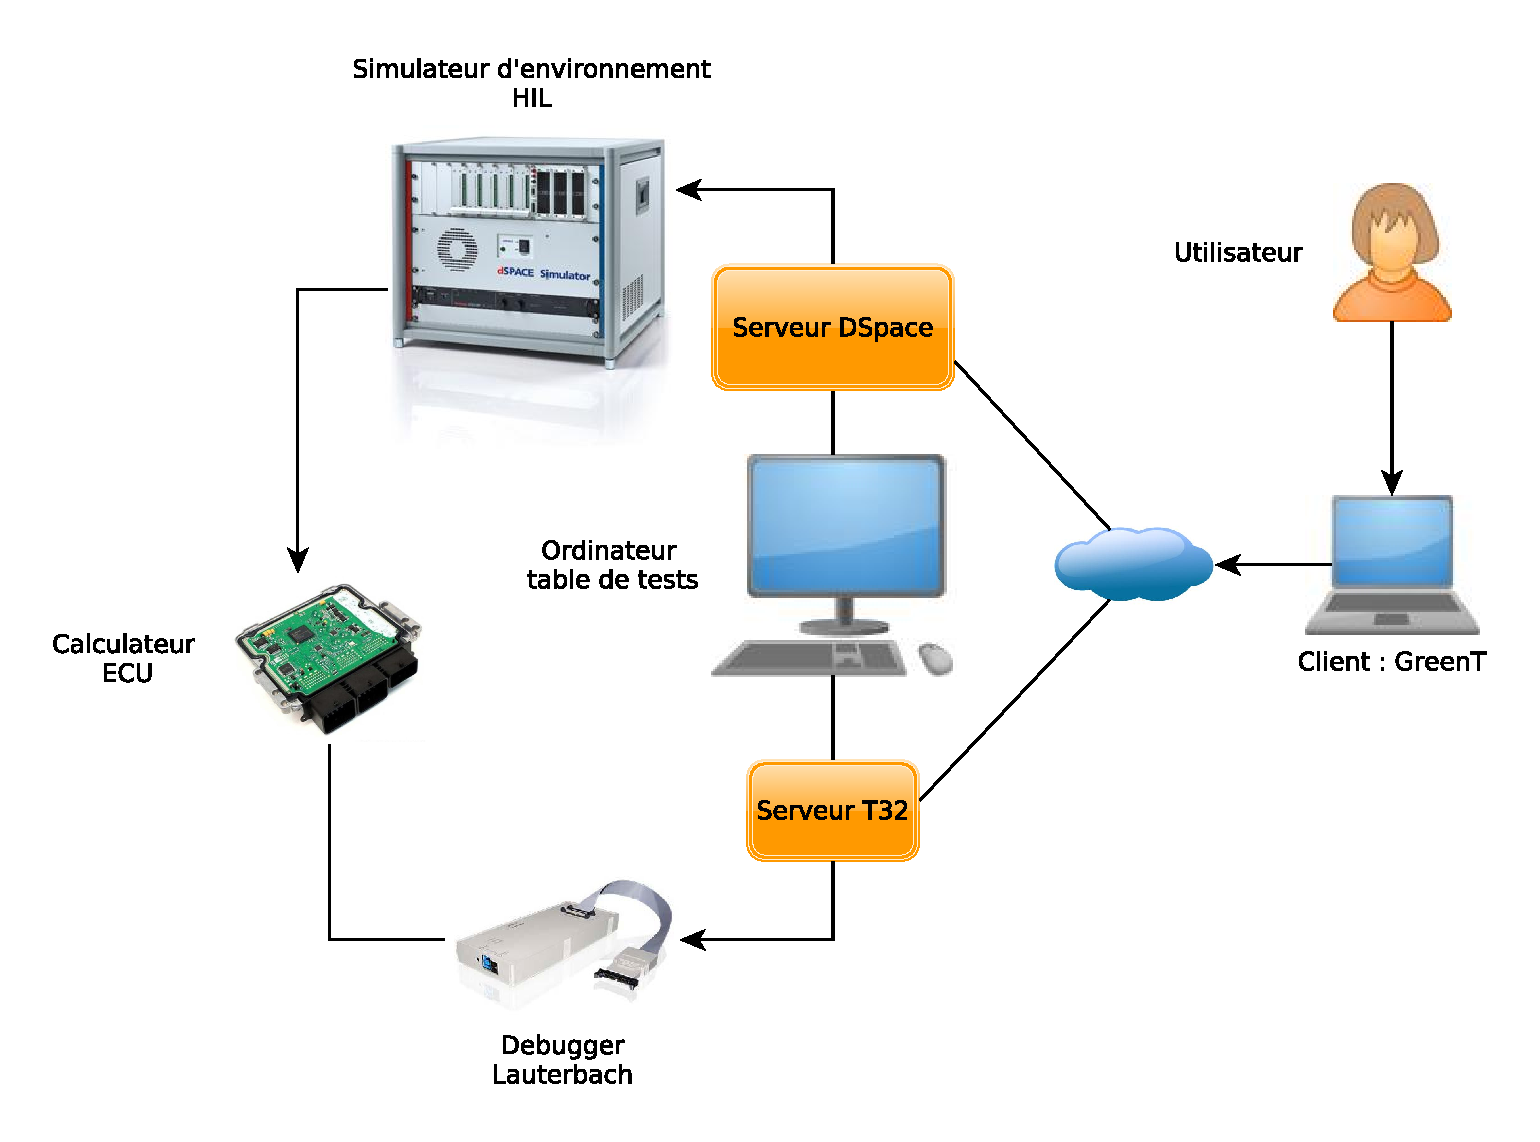
\includegraphics[width=\paperwidth]{images/network.eps}
	};
	\end{tikzpicture}
\end{frame}

\begin{frame}{Fonctionnement d'un cas de tests}
		  \setbeamercovered{transparent}
	\begin{itemize}[<+->]
	  \vfill
		\item Un scénario de précondition
		\begin{itemize}
			\item Initialise le banc de tests
		\end{itemize}
	\vfill
		\item Des scénarios de stimulation de l'environnement
			\begin{itemize}
			\item Pilotent le banc HIL 
			\item Enregistrement de variables durant les scénarios
			\end{itemize}
	\vfill
		\item \textit{Expected Behavior }
			\begin{itemize}
				\item Expression logique 
				\item Évaluée sur l'ensemble de l'enregistrement
			\end{itemize}
			\vspace{-30px}
	\end{itemize}
	\begin{figure}[H]
		\centering
		\only<1,2> {
			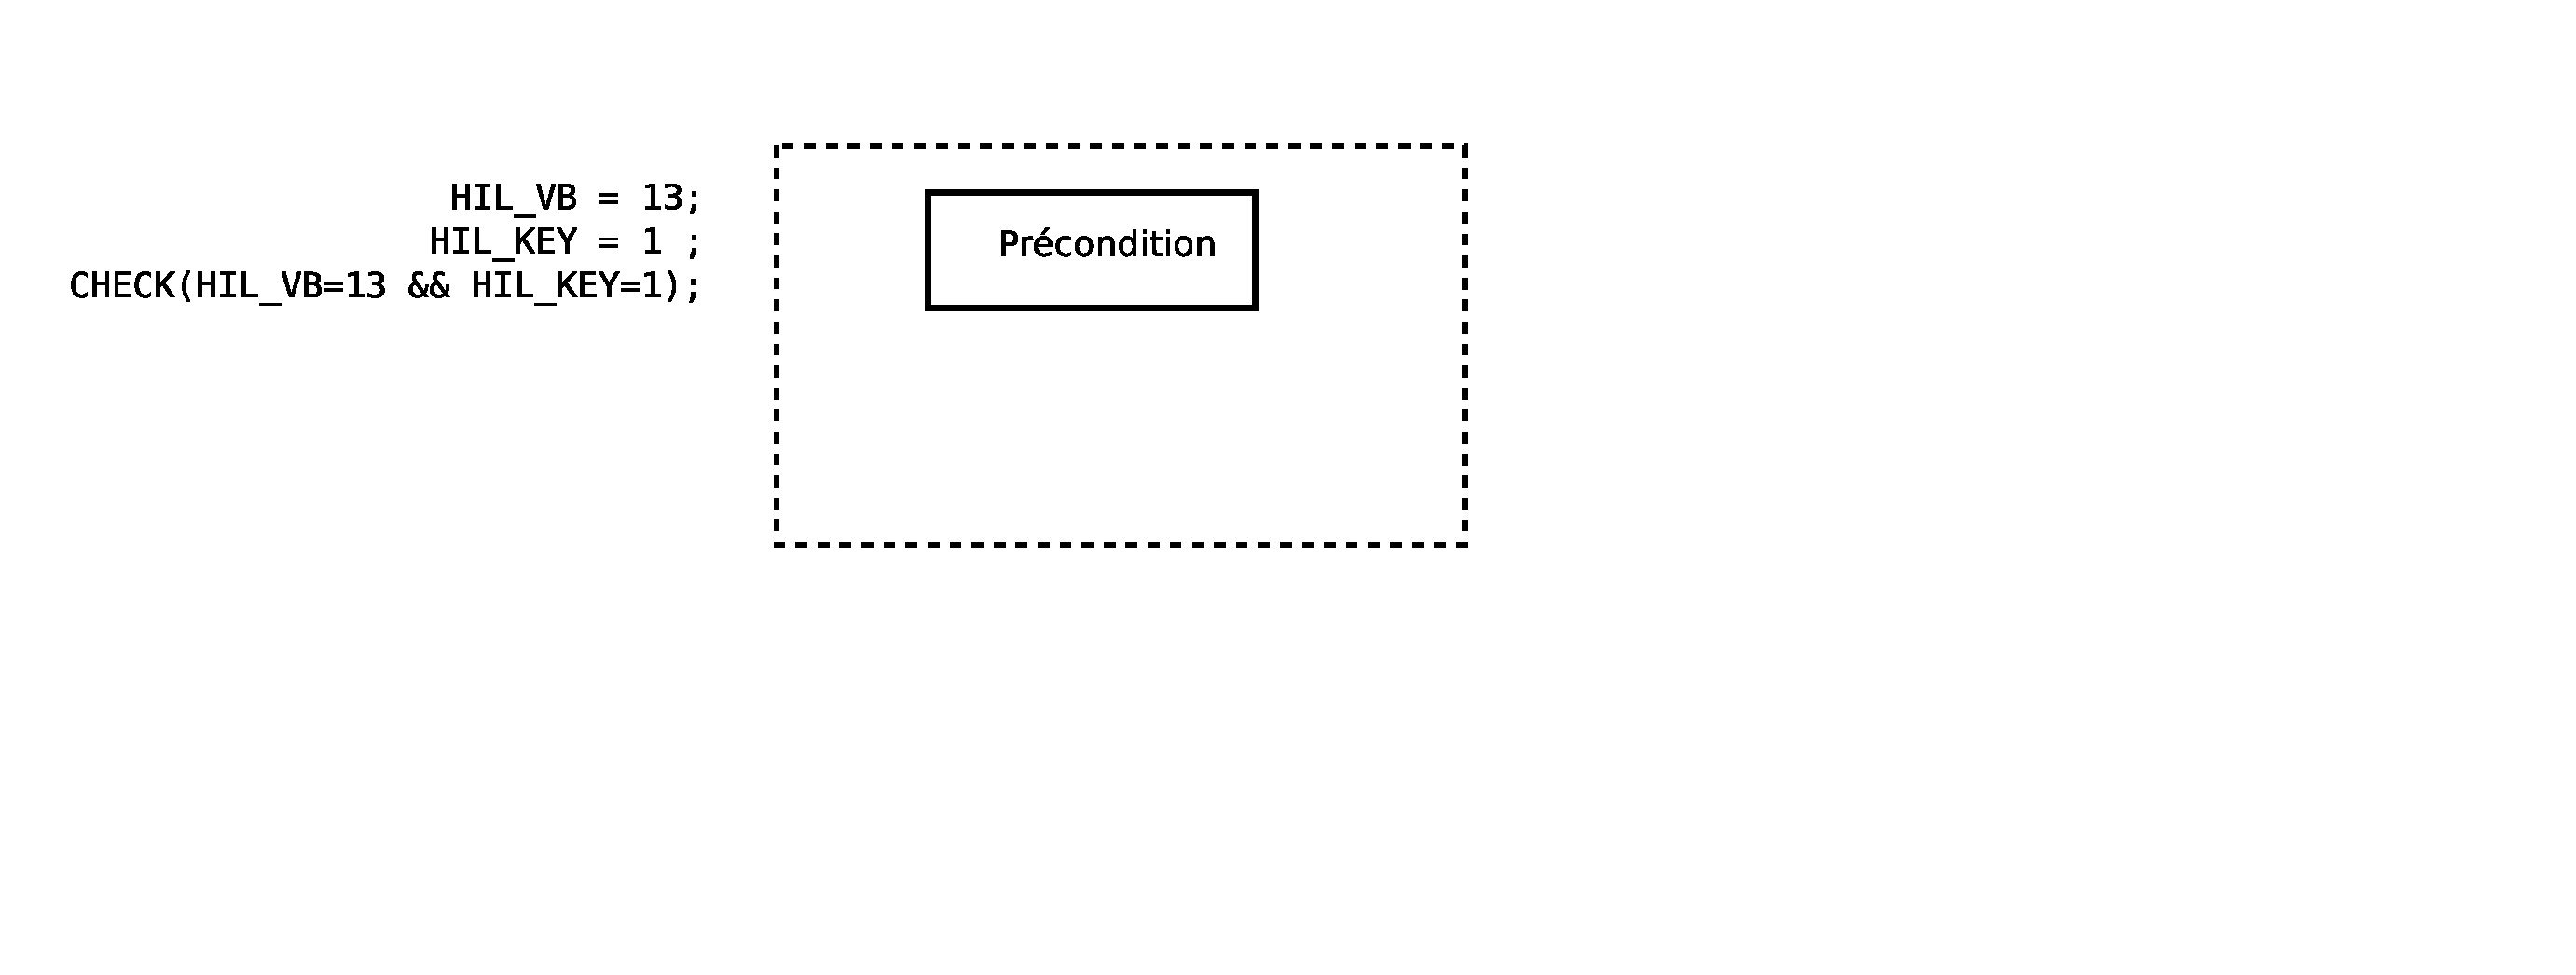
\includegraphics[width=9.5cm]{images/exe1.eps}
		}
		\only<3,4> {
			\includegraphics[width=9.5cm]{images/exe2.eps}
		}
		\only<5> {
			\includegraphics[width=9.5cm]{images/exe3.eps}
		}
		\only<6,7> {
			\includegraphics[width=9.5cm]{images/exe4.eps}
		}
		\only<8> {
			\includegraphics[width=9.5cm]{images/exe.eps}
		}
		\caption{Fonctionnement d'un exécutable}
	\end{figure}
\end{frame}




	\AtBeginSubsection[] {
		\begin{frame}<beamer>{Plan}
			\tableofcontents[currentsubsection]
		\end{frame}
	}
	\section{Travail réalisé}
	\subsection{La difficulté de production de rapports}
	\begin{frame}{Les tâches de calcul}
		% Récurrence
		% Variables d'entrées, de sorties

	\end{frame}
	\begin{frame}{\normalsize Problème de l'existant : échantillonnage trop rapide}
\begin{block}{Tâche de calcul}
			\begin{itemize}
				\item s'exécute dans une fenêtre temporelle
				\item récurrente
			\end{itemize}
		\end{block}
\begin{figure}
\centering
\includegraphics[width=1\linewidth]{images/badReport}
\caption{}
\label{fig:badReport}
\end{figure}
	\end{frame}

	\begin{frame}{\normalsize La solution : utilisation des variables de sorties}		
\begin{figure}
\centering
\includegraphics[width=0.9\linewidth]{../rapport/contents/images/goodReport}
\caption{}
\label{fig:goodReport}
\end{figure}

	\end{frame}
	\subsection{Les projets multi-cœurs}
	\subsection{La généralisation de l'outil}
	\subsection{La synchronisation des traces}
	\begin{frame}{Le besoin}
	\end{frame}
	\begin{frame}{\normalsize Première solution : un signal analogique, la batterie}
	\end{frame}
	\begin{frame}{\normalsize Seconde solution : un signal logique, la clé}
	\end{frame}
		
%\subsection{Développement}
\begin{frame}{L'état des lieux}
	\vfill
	\begin{itemize}
	\item Première version fonctionnelle livrée%~~~\Huge{1.0}
		\begin{itemize}
			\item Création de scripts de déploiement
			\item Rédaction du \textit{User Manual}
			\item Démonstration devant un responsable Allemand
		\end{itemize}
	\vfill
	\normalsize
	\item Utilisé sur projets Ford \textit{mono-core}%~~~ \includegraphics[height=1cm]{images/ford.png}
	\vfill	
	\item Rapports de tests au format Excel%~~~ \includegraphics[height=1cm]{images/excel.jpg}
	\end{itemize}
	\vfill
\end{frame}
\begin{frame}{La suite prévue du projet}
		\vfill
\begin{itemize}
	\item Effectuer des formations auprès des utilisateurs
	\vfill
	\item Assurer le support des utilisateurs
	\vfill
	\item Maintenance corrective
		\vfill
	\item Développement de nouvelles fonctionnalités
		\pause
	\begin{itemize}
		\item Adapter l'outil pour le \textit{multi-core}
		\item Amélioration graphique des rapports de tests
		\item Mettre en place un \textit{workflow} de développement
		\item Nouvelles demandes utilisateur\ldots
	\end{itemize}
\end{itemize}
	\vfill
% A effectuer
\end{frame}

	
\subsection{Méthodologie}
\begin{frame}{Méthodologie}
	\begin{figure}[H]
		\centering
		\includegraphics[height=1.5cm]{images/java.png}~~
		\includegraphics[height=1.5cm]{images/python.png}~~
		\includegraphics[height=1.5cm]{images/git.jpg}

		\includegraphics[height=1.5cm]{images/ecu.jpg}~~
		\includegraphics[height=1.5cm]{images/t32.jpg}~~
		\includegraphics[height=1.5cm]{images/dspace.jpg}
		\caption{Technologies et outils utilisés}
	\end{figure}
	\vfill
	\pause
\vspace{-20px}
	\begin{block}{Gestion de projet}
		\begin{itemize}
			\item Réunions régulières
			\begin{itemize}
				\item Hebdomadaire avec mon tuteur
				\item Mensuelle avec le chef de groupe
				\item Dès que nécessaire avec l'équipe cliente
			\end{itemize}

			\item Développement court et itératif\newline
				\footnotesize $\Rightarrow$ Le client sera au centre du développement
		\end{itemize}
			\end{block}
\end{frame}
\subsection{Objectifs}
\begin{frame}{Objectifs du stage} 
	\begin{block}{Objectifs personnels}
	\begin{itemize}
		\item Prise de responsabilité sur le projet
		\item Découverte du multi-core
		\item Analyse des premiers retours d'utilisateurs
		\item Analyse des nouveaux besoins
	\end{itemize}
\end{block}
\pause
\begin{block}{Objectifs pour l'entreprise}
	\begin{itemize}
		\item Démocratiser l'utilisation de l'outil
		\item Améliorer les tests d'intégration du plugin
		\item Gagner du temps 
	\end{itemize}
\end{block}
\end{frame}




	\sidetoc{no}
%	\section{} % 3'
	\begin{frame}{Bilan pour Continental}
	\begin{itemize}
		\item 2 campagnes de tests réalisées sur Ford Panther
		\begin{itemize}
			\item 8 bugs trouvés
			\item 300 tests rédigés par les utilisateurs\ldots 
			\item \ldots exécutés en 2h30
		\end{itemize}
		\pause
		\vfill
		\item 16 campagnes de tests prévues sur Ford Panther en 2017
				\pause
		\vfill		
		\item Début de généralisation de l'outil à Renault
		\begin{itemize}
			\item Nécessite la fin du développement de la synchronisation\newline
			$\Rightarrow$ Sera effectué d'ici fin Août
		\end{itemize}
				\vfill
	\end{itemize}
\end{frame}
\begin{frame}{Bilan Personnel}
	\begin{itemize}
		\item Connaissances du secteur de l'automobile
		\vfill
						\pause
		\item Vision d'un cycle de vie complet
		\begin{itemize}
			\item De l'analyse des besoins à l'exploitation
			\item Expérience en support et maintenance
		\end{itemize}
						\pause
		\vfill		
		\item Prise de responsabilités sur le projet
		\begin{itemize}
			\item Interface avec l'équipe client
		\end{itemize}
	\end{itemize}
\end{frame}


	% Slide for questions
	\begin{frame}{Avez-vous des questions ?}
		\begin{figure}[H]
			\centering
			\includegraphics[width=5cm]{images/interrogation.jpg}
		\end{figure}
	\end{frame}
\end{document}
